\documentclass[abstract=on,12pt]{scrreprt}

% Set packages to be used
\usepackage[hidelinks]{hyperref}	% Adds support for hyperlinks
\usepackage[british]{babel}			% Set the language to UK English
\usepackage[a4paper]{geometry}		% Set the paper type
\usepackage[T1]{fontenc}			% Change the encoding to allow for more character types
\usepackage{booktabs}				% More professional looking table layouts
\usepackage{etoolbox}				% Lets you do fancy stuff with section types
\usepackage{fancyhdr}				% Fancy Headers
\usepackage{graphicx} 				% For loading graphic files
\usepackage{multicol}				% Used to set column counts
\usepackage{pdfpages}				% Used to include external PDFs in the document
\usepackage{ragged2e}				% for '\RaggedRight' macro (allows hyphenation)
\usepackage{setspace}				% Sets the spacing between lines
\usepackage{tabularx}				% for 'tabularx' environment and 'X' column type
\usepackage{titlesec}				% Allows custom formatting for sections
\usepackage{apalike}				% Format references in APA styling
\usepackage{gensymb}				% Allow inclusion of special characters, such as degrees
\usepackage{lmodern} 				% Type1-font for non-english texts and characters

% Set document specific info
\title{Is Immersion Possible in Non-Euclidean Virtual Environments?}
\subtitle{CHP2524 - Individual Project Report}
\author{Nathan Boxhall-Burnett}
\setlength{\columnsep}{1cm}			% Set the spacing between columns
\onehalfspacing						% Set the spacing between the lines of text
\graphicspath{Images/}				% Set the default path to use for images

% Set the page number and running title as header
\pagestyle{fancy}
\fancyhf{}
\fancyheadoffset{0cm}
\renewcommand{\headrulewidth}{0pt}
\renewcommand{\footrulewidth}{0pt}
\fancyhead[R]{\thepage}
\fancyhead[L]{Is Immersion Possible in Non-Euclidean Virtual Environments?}
\fancypagestyle{plain}{%
	\fancyhf{}%
	\fancyhead[R]{\thepage}%
	\fancyhead[L]{Is Immersion Possible in Non-Euclidean Virtual Environments?}
}

% Set formatting for chapter titles
\titleformat{\chapter}[hang]{\huge\bfseries}{\thechapter}{1em}{\huge}

% Set formatting for section titles
\titleformat{\section}[hang]{\large\bfseries}{\thesection}{1em}{\large}

% Set formatting for section titles
\titleformat{\subsection}[hang]{\normalsize\bfseries}{\thesubsection}{1em}{\normalsize}

% Add the abstract to the table of contents
\patchcmd{\abstract}{\titlepage}{\titlepage
	\addcontentsline{toc}{chapter}{Abstract}}{}{}

% Begin the document
\begin{document}

	% Title Page
	\maketitle

	% Set the inital pages to use roman numerals for numbering
	\pagenumbering{roman}

	% Table of contents
	\tableofcontents

	% Abstract
	\begin{abstract}
		\thispagestyle{plain}
		expression of general problem/area

		specific problem/objective attempted

		what you have achieved

		lessons learned

		%% DO NOT START BY SAYING WHAT YOU HAVE DONE 
		%% DO NOT INCLUDE JARGON / DETAILS 
		% Eg bad start “I have implemented a C\# database running on Linux v4.5.2 … “
		% Eg bad start “ I have created a web application” – start with overview and problem area first.
		%% MAKE IT UNDERSTANDABLE TO ALL ! 


%		With Virtual Reality (VR) development and availability increasing as rapidly as it has in recent years, especially in the video game market, experiences that are capable from Virtual Environments (VE) that are not limited to the restrictions of the real world, and the effectiveness they have in a users perception, need to be considered.
%		This review explores the existing literature that covers the various requirements for creating a VE that consumers would perceive as 'realistic' in VR. As well as this, it also covers how these requirements have been, and can, be adapted to work inside of a world which does not follow the restrictions of real world geometry, such as in non-Euclidean or Escheresque space.
%		Gaps in the current literature are outlined, alongside perspective areas for future research.
	\end{abstract}

	% Set formatting for section titles
	\titleformat{\chapter}[hang]{\large\bfseries}{\thechapter}{1em}{\large}

	% Remove section numbering for the acknowledgements
	\setcounter{secnumdepth}{-2}

	% Document Acknowledgements
	\chapter{Acknowledgements}
		I would like to thank my supervisor Hugh Osborne, and examiner Duke Gledhill, for their invaluable feedback and suggestions throughout.
		I would also like to thank all the participants who took the time to take part in the product experiments.

	% Set formatting for chapter titles
	\titleformat{\chapter}[hang]{\huge\bfseries}{\thechapter}{1em}{\huge}

	% Reset the page count, reset the numbering style to arabic, and add section numbering again
	\newpage
	\renewcommand\thepage{\arabic{page}}
	\pagenumbering{arabic}
	\setcounter{secnumdepth}{3}

	% Introduction
	\chapter{Introduction}
\label{intro}

%explains  context, the problem/area, the clients / users / target audience. Also it should give a summary of what you have achieved and what your deliverable is.

%% HINT: Start by introducing the reader to the area, then explain what the specific problem/area you have tackled is and then what you have achieved.
%% MAKE IT CLEAR WHAT YOU HAVE DONE/ACHIEVED
%% COMPLETE YOUR INTRODUCTION AFTER YOU HAVE FINISHED THE REST OF THE PROJECT REPORT!



%Here I will be introducing the project and the various sections of the report document in detail, making sure to cover the terms and concepts that will be discussed to ensure the reader has full understanding of the report contents.

	% Literature Review
	\chapter{Literature Review}

	% Intro Page
	\section{Introduction}
\label{lr:intro}
%	Here I will be introducing and outlining the concepts that will be covered in the following sections.
	
	Virtual Reality (VR) is fast becoming a mainstream platform for video games, with high quality devices allowing the feeling of \enquote{presence} in a game world being released for computers, game consoles, and mobile devices alike, creating a vast user base for potential products.

	As well as this, the popularity of video games which utilise non-standard or real-world geometric principles are also increasing, with the popularity of titles such as Antichamber \cite{Antichamber2013} and Portal 2 \cite{Portal22011} engaging consumers with their non-conformity to the physics and geometry of average game worlds.

	This review explores the existing literature that covers the various requirements for creating a VE that consumers would perceive as \enquote{realistic} in VR.
	As well as this, it also covers how these requirements have been, and can be, adapted to work inside of a world which does not follow the restrictions of real world geometry, such as in non-Euclidean or Escheresque space.
	Gaps in the current literature are outlined, alongside prospective areas for future research.

	This review is split up into three chapters, each one covering a specific area of existing literature relevant to it:
	\begin{enumerate}
		\item \nameref{lr:vr}, which will cover various elements creating a sense of presence in a Virtual Environment (VE) using VR requires, such as user perception and affordances
		\item \nameref{lr:ne}, which will cover existing applications of non-standard geometry in video game systems
		\item \nameref{lr:cross}, which will cover how the requirements from the previous chapters are to be utilised together to form a working system, as well as the tools which are best suited for constructing such a system
	\end{enumerate}


	% Requirements for Presence in Virtual Reality chapter
	\section{Presence in Virtual Reality}
\label{lr:vr}
	
	\subsection{Introduction}
	\label{lr:vr:intro}
	%		This section will introduce the key concepts that will be discussed in the following subsections.
		Presence is the term used in VR systems to describe a user's sense of existing inside a VE. Because of this, it can be seen as one of, if not the most important feature of the design for a VR system.

		There are a few main features which are key to achieving a sense of presence in a VE. One example would be the general perception of the user for things such as depth perception, the ability for a person to calculate the distance of a point from themselves, and sensorimotor adaptation, which is the calibration of a user's senses to fit their environment.
		As well as this, there are specified areas such as affordance detection, the ability for a person to calculate interaction with an object or environment, which helps assist a user with navigation and interaction in a VE.
		The following sections will review existing literature on the aforementioned features.
	
	\subsection{Affordances in VR}
	\label{lr:vr:affordances}
	%		Here I will introduce the concept of, and cover research into affordances in Virtual Reality.
		%Perceiving affordances in virtual reality: influence of person and environmental properties in perception of standing on virtual grounds
		Affordance is especially important to get right in VR, particularly in a video game environment, due to the world a user is in is designed to be interacted with.
		Unlike what common sense would dictate, research on affordance in the real world may not be as applicable for when designing interactions in a virtual world as expected.
		A study \cite{Regia-Corte2012} focusing on a person's perception for whether or not they could stand upright on an object at various angles in a virtual world found that, contrary to expected results, users would tend to be more cautious when judging their ability in a virtual environment (critical angle 21.98\degree) compared to an equivalent object in the real world (critical angle 30\degree), even with a lack of apparent risk.

		This study covered the various requirements for the experiments well, however there were a few areas in which it could still be expanded upon.
		These areas include comparing results from using a variety of VR systems to judge responses based on hardware response times, display resolutions, and refresh rates, as well as increases and decreases in model and texture quality (not just the texture itself as they did) for judging the surfaces of the objects.

		% Designing presence for real locomotion in immersive virtual environments: an affordance-based experiential approach
		Another way in which affordance directly affects a user's sense of presence in VR is the simulation of real locomotion for the user.
		In a study \cite{Turchet2015} covering the ways in which a user's movement is recorded and displayed in a VE (including, but not limited to, individual foot tracking, arm, leg, and head tracking, movement speed tracking, etc.), results found that while an increase in the coverage of the input also increased the sense of presence for the user, it was more important to focus the areas based on their relevance to the scenario at hand.
		As well as this, the study found that while the input tracking itself was important, to attain a greater sense of presence it was also required for the physical representation of the user to match their real physical selves as much as possible, such as gender, height, and weight.

		This study, while extremely thorough in its coverage of the various possible elements required to generate a sense of presence, could have recorded and displayed its results in a more usable manner than it did.
		Due to the way the experiments were conducted, the results do not indicate any sense of importance for each individual step in its contribution to the feeling of presence in the user.
		Because of this, further research could be undertaken to create a weighted system designed around the experiments conducted, signifying its importance for specific VR systems, creating a more convenient set of data for future use.

	\subsection{Perception in Virtual Environments}
	\label{lr:vr:perception}
		%This section will cover existing research into how people perceive environments in Virtual Reality.
		% Using virtual reality to augment perception, enhance sensorimotor adaptation, and change our minds.
		Perception is a key feature to get right in VR, as incorrect calibration for features such as head tracking and input response can have both unintended, and undesired side-effects. In studies \cite{Wright2006}  \cite{Wright2009} \cite{Wright2011} \cite{Wright2013} \cite{Wright2014} around the effects of perception augmentation and sensorimotor adaptations, results showed that tests around sensorimotor processes that made use of Virtual Reality systems could have both intended and unintended effects on the participants central nervous system. 
		(NOTE) This paragraph needs expanding upon


		% Immersive Virtual Environment Technology to Supplement Environmental Perception, Preference and Behavior Research: A Review with Applications

		(PLACEHOLDER) Discuss \cite{smith2015} - Immersive virtual environment technology to supplement environmental perception, preference, and behaviour research

	\subsection{Conclusion}
	\label{lr:vr:conclusion}
		%Here I will summarise the concepts and sources discussed in the previous sections, how reliable they may be, and how the concepts could apply to my project.
		Due to recent relevant technology being both of a high quality, and low enough cost to warrant consumer interest, as well as its applications in not just Video Games, but in Medicine, Psychology, and Education, Virtual Reality is a very highly researched area.

		Studies have been conducted to cover an extremely wide range of applications and effects for VR, and because of this, there is a very solid foundation of work which can be both applied for practical uses, as well as a platform to build upon for future research.

		This is especially true in the two main focus points for the literature covered in this review, and will be beneficial for reference during the creation of the proposed system.


	% Non-Standard Geometry chapter
	\section{Non-Standard Geometry in Game Engines}
\label{lr:ne}

	\subsection{Introduction}
	\label{lr:ne:intro}
%		In this section I will introduce the concept of non-standard geometry, e.g. non-Euclidean, and review existing literature regarding its use in video game engines.
	
	\subsection{Existing Examples}
	\label{lr:ne:existing}
%		Here I will cover literature around non-Euclidean geometry, as well as existing examples of such geometry in virtual environments.
		(PLACEHOLDER) The following sources will be discussed in this section:
		\begin{itemize}
			\item \cite{Maric2014} - Formalizing complex plane geometry
			\item \cite{Turner2009} - Mathematics and the Imagination
			\item \cite{Lindley2005} - Game space design foundations for trans-reality games
		\end{itemize}
		
	\subsection{Conclusion}
	\label{lr:ne:conclusion}
		%This section will be used to sum up the sources discussed above, how relevant and reliable they are as sources, and how they relate to my project.


	% Application of Virtual Reality in a Non-Euclidean world Chapter
	\section[Non-Standard Geometry in Game Engines, and VR Applications]{Non-Standard Geometry in Game Engines, and the Application of VR in Non-Euclidean worlds}
\label{lr:cross}

	% In this section I will introduce the concept of non-standard geometry, e.g. non-Euclidean, and review existing literature regarding its use in video game engines.
	
	% In this section I will introduce the concepts to be covered in this section, namely how one can apply the key concepts for perception and presence in VR to a game world using non-standard geometry.

	\subsection{Existing Examples}
	\label{lr:ne:existing}
	
	% So yeah, here you'll just need to talk about how there really isn't any existing literature regarding non-Euclidean geometry in virtual environments. probably a good idea to mention how this is not a bad thing, as it means there is plenty of room for the project, and makes the project worthwhile?

		% Here I will cover literature around non-Euclidean geometry, as well as existing examples of such geometry in virtual environments.
		(PLACEHOLDER) The following sources will be discussed in this section:
		\begin{itemize}
			\item \cite{Maric2014} - Formalizing complex plane geometry
			\item \cite{Turner2009} - Mathematics and the Imagination
			\item \cite{Lindley2005} - Game space design foundations for trans-reality games
		\end{itemize}
	
	\subsection{Application}
	\label{lr:cross:application}

%		Here I will be covering any existing research which relates to the combination of VR and non-Euclidean geometry.
		(PLACEHOLDER) The following sources will be discussed in this section:
		\begin{itemize}
			\item \cite{Cruz-Neira1993} - Surround-screen projection-based virtual reality
			\item As referenced in \ref{lr:vr:perception}, \cite{Wright2014} - Using virtual reality to augment perception, enhance sensorimotor adaptation, and change our minds - Discuss how it could also relate to sensorimotor adaptations allowing a user to get accustomed to existing i\textsl{}n a non-Euclidean world.
		\end{itemize}
	
	\subsection{Tools \& Techniques}
	\label{lr:cross:tools}

%		This section will cover tools which are applicable for the creation of VR/Non-Euclidean virtual environments.
		(PLACEHOLDER) In this section I will be covering the various tools I could use to create the proposed system, these tools and techniques will include:
		\begin{itemize}
			\item Software 
			\begin{itemize}
				\item Custom engine
				\begin{itemize}
					\item Oculus SDK 0.8
					\item NVIDIA Gameworks VR
					\item AMD LiquidVR
					\item DirectX 11.2 / 12
					\item OpenGL 4.5
				\end{itemize}
				\item Modify existing engine
				\begin{itemize}
					\item Unity 5
					\item Unreal 4
				\end{itemize}
			\end{itemize}
			\item Hardware
			\begin{itemize}
				\item Head-Mounted Display
				\begin{itemize}
					\item Oculus Rift DK2
					\item HTC Vive
				\end{itemize}
				\item Input
				\begin{itemize}
					\item Keyboard/Mouse
					\item Game controller (PS4, XBox One, etc.)
					\item Web-cam/Kinect
				\end{itemize}
			\end{itemize}
			\item Project Management
			\begin{itemize}
				\item Time Planning
				\begin{itemize}
					\item Agile
					\item Waterfall
				\end{itemize}
				\item Source Control
				\begin{itemize}
					\item Git
					\item SVN
				\end{itemize}
			\end{itemize}
		\end{itemize}
		Resources for reference:
		\cite{Bruce2012} - Custom engine v modify an existing one - debate. Compares the pros and cons of both modifying an existing engine and creating a custom solution. ('Leaky Abstractions' with an existing engine, balance engine efficiency and actual system development with a custom engine, etc.).
		
	\subsection{Summary}
	\label{lr:cross:conclusion}
		% There is a severe lack of academic research into non-standard geometry in virtual environments
%		This section will sum up the points discussed in the above subsections.
		(PLACEHOLDER) Sum up the points discussed in the above sections. Example: current implementations of non-euclidean geometry in released games have always directly used, or modified an existing generic game engine to create the VE, and are therefore not optimised to be used in a non-euclidean world.


	% Conclusion
	\section{Conclusion}
\label{lr:conclusion}

	In Virtual Reality, non-standard geometry is definitely an area with potential to engage, and possibly spark an interest within a user about the capabilities and uses of such concepts.

	% TODO - Reword this?
	This review has given an overview into the various components required for the creation of an environment suitable for use in VR, how non-standard geometrical worlds can be created for use in a VE, and how the areas both require adaptation in order to work together.

	In terms of VR, existing literature is very thorough in its coverage of the possibilities and effects of its use both within and outside of video game environments.
	Several key areas that should be considered when designing a virtual environment for VR were outlined such as affordance detection and potential sensorimotor adaptation, and how they can effect a users sense of presence and immersion.
	Although there is definitely still room for further research into the more niche areas of study, there is a solid foundation for use as a reference for further development in the field.

	For non-Euclidean geometry, however, there is a distinct lack of academic research into its use within virtual environments, with most studies focusing instead on the theoretical applications for it.
	Reports around the use of non-standard geometry in video games does exist, however due to the non-scholarly nature of the sources, which are mainly video game journalist articles or developer interviews, they cannot be completely trusted for academic purposes.

	Due to combination of the findings surrounding these areas, research into the use of non-Euclidean geometry within a VR system is very open to exploration, and as such, research would be beneficial as a possible basis for further study, perhaps even encouraging it.


	% Maybe other background stuff too, who knows

	% Models/Product Design stuff
	\chapter[Product]{Design and Implementation}
\label{design}

	\section{Introduction}
	\label{design:intro}

		Due to the room for research available in this area, it made sense to focus this study on a relatively broad area of the subject to be used as a foundation, rather than to specialise on a particular niche.
		% REWORD THIS?
		Because of this, the main focus for this study is the effects that Non-Euclidean geometry has on a user's sense of Immersion, and to find any changes in a user's comfort navigating in a virtual environment.

		This chapter covers the development process that was undertaken for the creation of the product used for the experiments.

	\section{Development Process}
	\label{design:dev}

		% THIS section will cover the development process of the product itself

		% Talk about development methodologies considered for use with the project, and how they were adapted for use for a single person.
			% Use of Git and stuff like that

		% Talk about how you decide to use an existing engine you knew well (save time reinventing the wheel for things like lighting, camera stuff, etc)
		% Also you wanted to limit the amount of outside variables as possible, so an existing engine helped with that

		% Talk about implementation process
			% Started off using render textures, but that had problems regarding depth perception, outside of VR it was fine but inside it was obviously a plane
			% Changed to using render culling and directly viewing the cameras with a bit more tranlation and rotation magics
			% Challenge with multiple variations in how the areas can be set up - angles, inversions on both sides, whether one or both should render, whether you should be able to use it to transport, etc


	\section{Product model}
	\label{design:model}

		% THIS section will contain models of the various states and relations between the functions and other workings of the product, for areas such as the transition between non-Euclidean world areas.
		\autoref{appendix:code:camera} \autoref{appendix:code:player}

	\begin{figure}[H]
		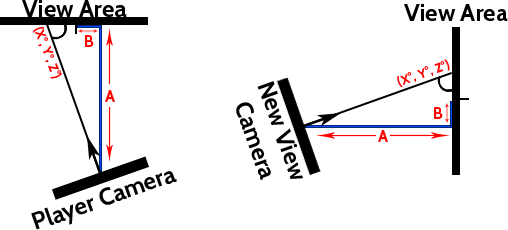
\includegraphics[width=0.8\textwidth]{Images/Position}
		\centering
		\caption{2D representation of the calculations for the position and rotation of cameras.
			See \autoref{appendix:code:camera} for the implementation}
		\label{design:fig:maths}
	\end{figure}

	\begin{figure}[H]
		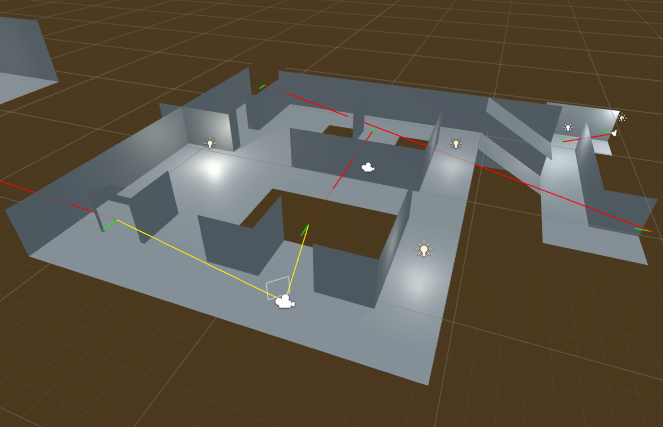
\includegraphics[width=1\textwidth]{Images/Lines_Everywhere2}
		\centering
		\caption{Example view of a scene.
			Red lines are connections between points,
			yellow lines are connections visible to the player,
			and green lines are the direction the connectors are facing}
		\label{design:fig:scene}
	\end{figure}

	\begin{figure}[H]
		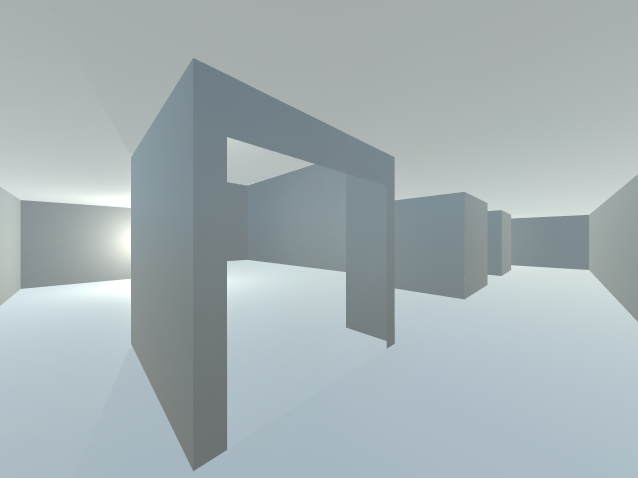
\includegraphics[width=1\textwidth]{Images/NE_View}
		\centering
		\caption{Example of view from inside the Non-Euclidean scene, displaying an area which is larger on the inside}
		\label{design:fig:game}
	\end{figure}

	\section[Environment Design]{Design of experiment environments}
	\label{design:design}

		The design of the environments to be used in the experiments is almost as important as the functionality of the system itself, as it is the only medium through which the participants will be able to provide feedback.
		Two separate scenes were created for use in the experiments, one where the participants would be navigating through a non-Euclidean environment, and the other which would only make use of standard Euclidean space. % TODO: Reword this?

		To limit the number of factors which could affect the immersion of a participant in the experiments, a minimalistic aesthetic was chosen for the scenes.
		By using simple white texturing and relying on lighting for definition, impurities that could be noticed by pixelation of detailed textures were removed, focusing the participant's attention solely on the geometry of the scenes.
		Similarly, the scenes themselves were modelled using simple primitive shapes, such as planes and cubes, to try and minimise any impacts in immersion that could be caused by low polygon counts in more complex models.
		Testing was done on scenes which used more detailed textures (\autoref{design:fig:design:tex}), however any imperfections in the scene were much more apparent in this scene compared to the minimalistic designs of the completed experiment scenes.

		\begin{figure}[h]
			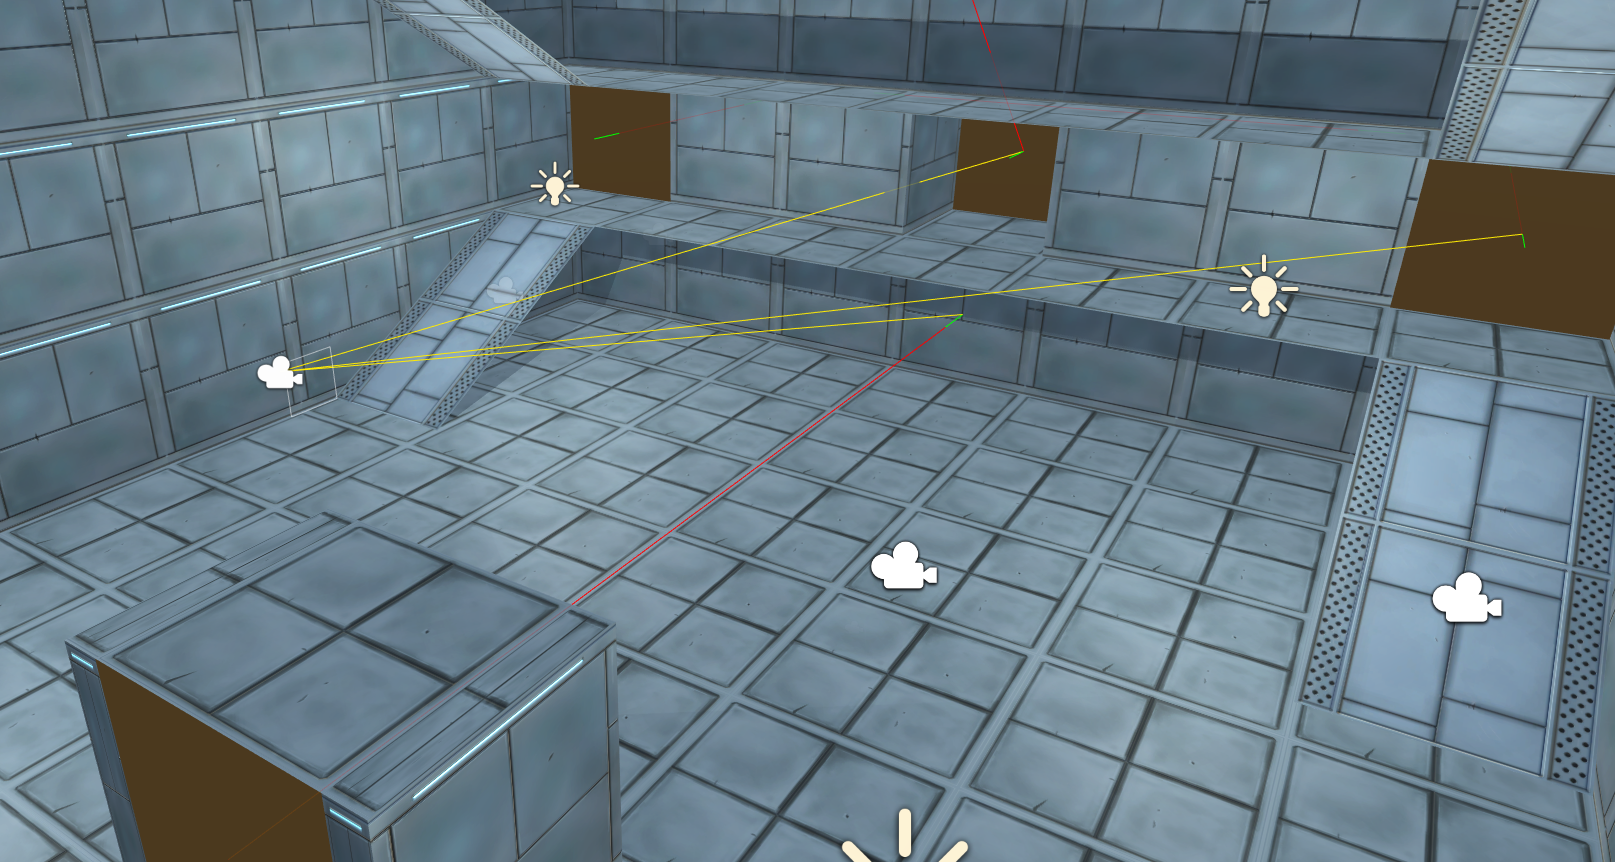
\includegraphics[width=1\textwidth]{Images/Lines_Everywhere}
			\centering
			\caption{Test scene using textured objects}
			\label{design:fig:design:tex}
		\end{figure}

		\subsubsection{Non-Euclidean Scene}

			The non-Euclidean test scene (as seen in \autoref{design:fig:design:ne}) was the first of the two scenes to be designed for the experiments.
			As a way to ensure the participants could experience a variety of the possibilities of non-Euclidean environments, a mixture of effects were chosen to be included in the scene, as labelled in \autoref{design:fig:design:ne} by the letters and corresponding red lines.

			\begin{figure}[h]
				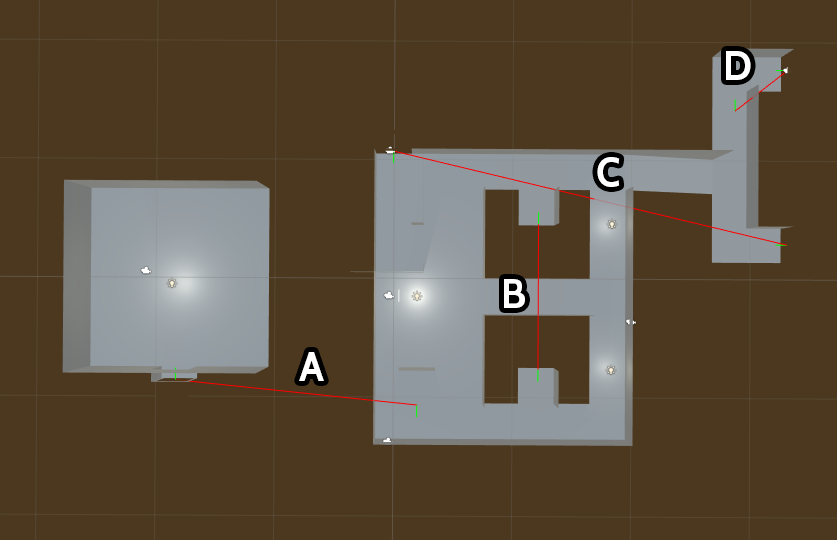
\includegraphics[width=1\textwidth]{Images/NE_Layout}
				\centering
				\caption{Labelled layout of the Non-Euclidean experiment scene}
				\label{design:fig:design:ne}
			\end{figure}

			Point \enquote{A} represents the connection shown in \autoref{design:fig:game}, which is an example of an area appearing to contain a larger area than expected from its surroundings.
			Connection \enquote{B} represents what appears to be a direct corridor to a user which both takes a shorter path than would be expected by the two parallel paths, but also appears to occupy the same space as another corridor which runs perpendicular to it.
			Connection \enquote{C} appears to a user that they are able to walk directly between two completely separate areas of the room, both of which are on different levels (Note the corridor to the right of the \enquote{C} marker is a ramp leading down towards \enquote{D}).
			Finally, connection \enquote{D} gives the impression that the user is walking around a seemingly endless series of turns, however when the user turns back from where they came from, they find they have not travelled anywhere.

			The ramp connecting the two levels in the scene (As seen between points \enquote{C} and \enquote{D} in \autoref{design:fig:design:ne}) is at an angle of 20\degree, below the 21.98\degree critical angle for perceiving affordance when in VR \cite{Regia-Corte2012}.

		\subsubsection{Standard Scene}
			The standard Euclidean scene (as seen in \autoref{design:fig:design:standard}) was designed to follow a similar layout to the non-Euclidean one, or as close as could be possible with the geometric constraints.
			This decision was made to attempt to limit the factors that could affect the participant's immersion within the scenes, as a way to ensure that the results from the experiments are as consistent as possible.

			\begin{figure}[H]
				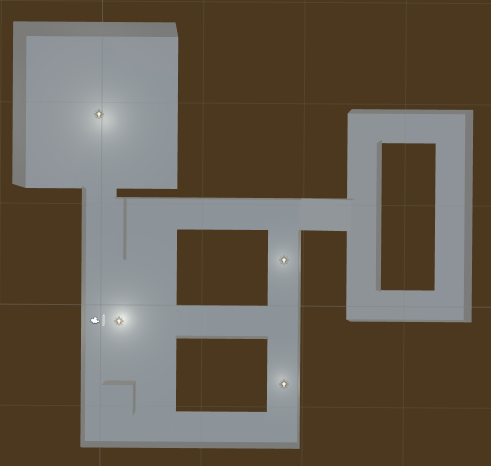
\includegraphics[width=0.7\textwidth]{Images/Standard_Layout}
				\centering
				\caption{Layout of the standard Euclidean experiment scene}
				\label{design:fig:design:standard}
			\end{figure}


	% Experiment
	\chapter[Experiment]{Experiment Evaluation}
\label{exp}

	\section{Introduction}
	\label{exp:intro}

		As a way to get the widest possible range of data from the scenes created, two different experiments were planned (\enquote{Experiment 1}, and \enquote{Experiment 2}).
		The experiments were set up in a way that a participant in an experiment would either be shown the standard or non-Euclidean game scene first, and once they had successfully navigated around it, they would then be shown the other.
		\enquote{Experiment 1} had the participants viewing the standard scene first and the non-Euclidean scene second, with \enquote{Experiment 2} having the participants view the non-Euclidean scene first and the standard scene second.

		A total of 10 participants took part in the experiments, with 5 participants taking part in \enquote{Experiment 1}, and the other 5 \enquote{Experiment 2}.
		Having the participants view the two scenes in different orders allowed for the results of the experiments to not only cover the effects of the respective scenes geometry, but also to see if being exposed to the other environment in any way impacts their immersion to the one they are currently in. % TODO: Reword this

		During the experiments, participants were asked to fill out a 2 page questionnaire, a blank version of which can be seen on page \pageref{appendix:question}.
		After viewing the first scene, participants were asked to fill out the first page of the questionnaire. Once they'd filled the page, they would view the second scene, after which they were asked to fill out the second page. % TODO: Reword this

		The analysis of the gathered results will be covered in three sections. The first will cover the results from all 10 experiments solely on the data gathered for the standard scene; The second covers the results from all 10 experiments solely on the data from the non-Euclidean scene; Finally, the third covers the comparison between the two scene types depending on the order of viewing. % TODO: Reword this?

		% REMEMBER TO SPEAK ABOUT THE MATHS

	\section{Experiments}
	\label{exp:exp}

		\subsection{Standard Euclidean Geometry}
		\label{exp:exp:standard}

			Having an experiment scene using standard Euclidean geometry which follows a similar layout to the non-Euclidean scene sets a good foundation for the validation of the results. % TODO: Reword this?
			The questionnaire the participants were asked to fill in focused on two main metrics, their personal sense of immersion within the scene, as well as their sense of comfort navigating the scene.

			% Talk about the results specific to the standard euclidean geometery here.
			% Used to get a base result for immersion
			% Consistent high ratings for immersion
			% Navigation comfort was varied, but talk about the high mean values

			% IMMERSION MEAN: 7
			% COMFORT MEAN: 7

			\begin{figure}[H]
				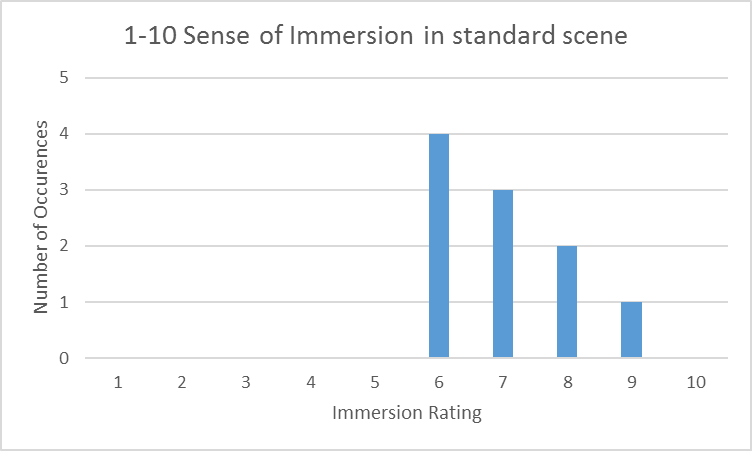
\includegraphics[width=0.7\textwidth]{Images/Standard_Immersion}
				\centering
				\caption{Immersion rating in standard geometry test scene}
				\label{exp:fig:standard_immersion}
			\end{figure}

			\begin{figure}[H]
				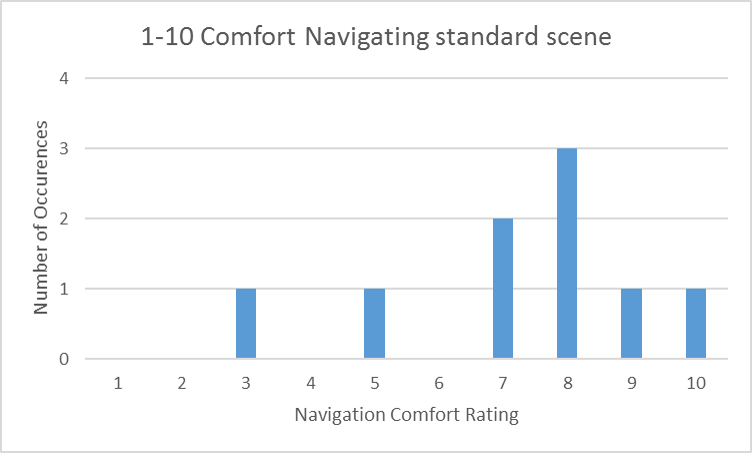
\includegraphics[width=0.7\textwidth]{Images/Standard_Comfort}
				\centering
				\caption{Navigation Comfort rating in standard geometry test scene}
				\label{exp:fig:standard_comfort}
			\end{figure}

			\begin{figure}[H]
				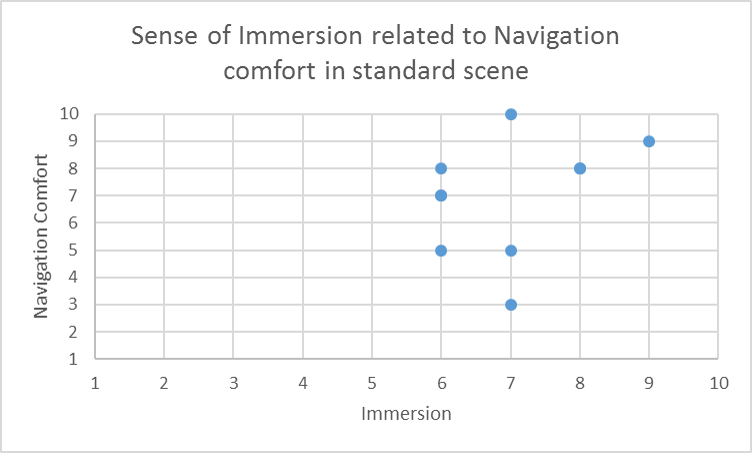
\includegraphics[width=0.7\textwidth]{Images/Standard_Relation}
				\centering
				\caption{Relation between sense of immersion and navigation comfort in standard geometry test scene}
				\label{exp:fig:standard_relation}
			\end{figure}

		\subsection{Non-Euclidean Geometry}
		\label{exp:exp:ne}

			Similarly to the standard Euclidean scene, after viewing the non-Euclidean scene participants were asked to answer questions relating to two main metrics, their sense of immersion, and comfort navigating the scene.

			% Talk about the results specific to the non-eucldean geometry here
			% More varied results
			% Same Mean
			% More responses in the higher end of the scale - talk about the written feedback
			% Lower comfort with navigation

			% IMMERSION MEAN: 7
			% COMFORT MEAN: 6.2

			\begin{figure}[H]
				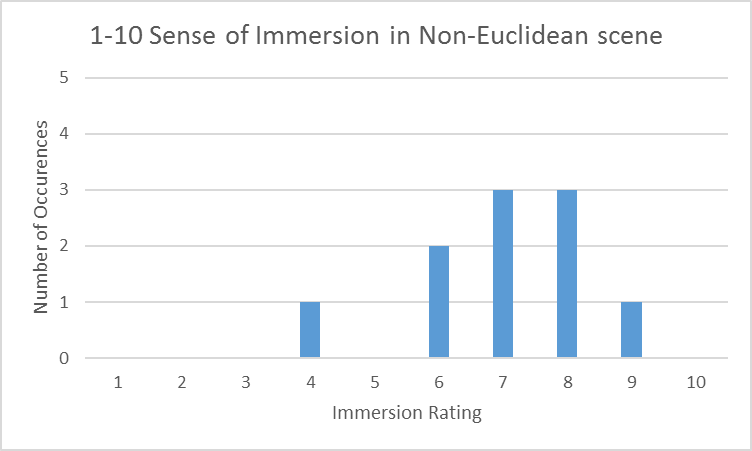
\includegraphics[width=0.7\textwidth]{Images/NE_Immersion}
				\centering
				\caption{Immersion rating in Non-Euclidean geometry test scene}
				\label{exp:fig:ne_immersion}
			\end{figure}

			\begin{figure}[H]
				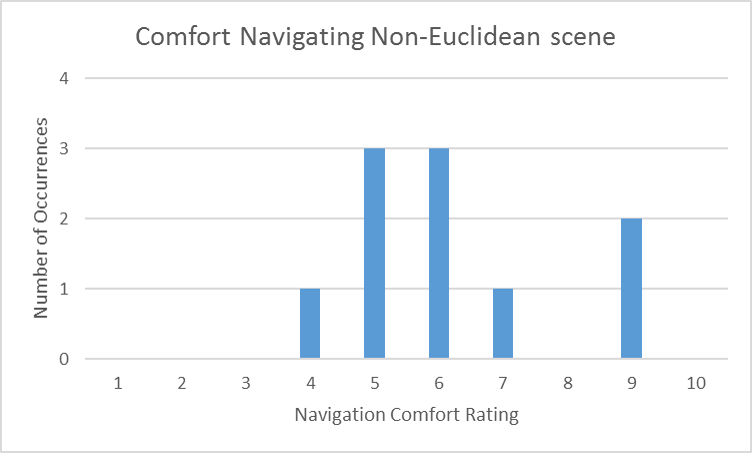
\includegraphics[width=0.7\textwidth]{Images/NE_Comfort}
				\centering
				\caption{Navigation Comfort rating in Non-Euclidean geometry test scene}
				\label{exp:fig:ne_comfort}
			\end{figure}

			\begin{figure}[H]
				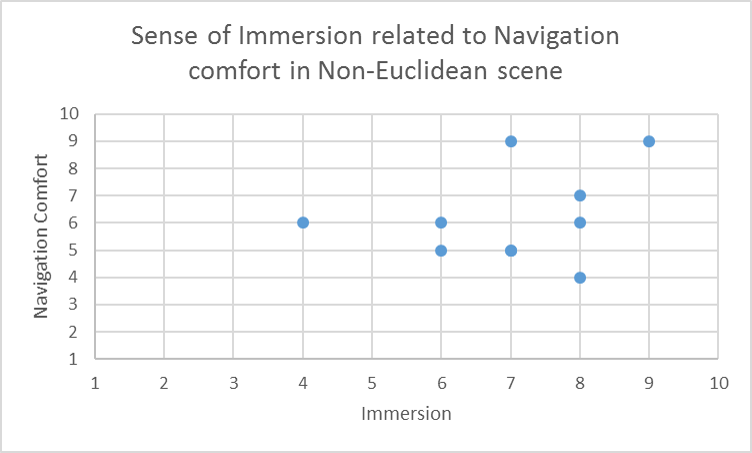
\includegraphics[width=0.7\textwidth]{Images/NE_Relation}
				\centering
				\caption{Relation between sense of immersion and navigation comfort in Non-Euclidean geometry test scene}
				\label{exp:fig:ne_relation}
			\end{figure}

		\subsection{Comparisons}
		\label{exp:exp:comp}

			With the results of both individual scenes gathered and analysed, 

			% Experiment 1 was Standard First
			% Experiment 2 was NE First
			% Talk about the comparisons
			% Talk about how the data MEANs something
			% Participants from exp1 never felt that NE was less immersive, either as immersive or more - quote feedback - \enquote{The puzzling nature of exploring a familiar map that is no longer familiar} was a positive impact on immersion
			% Participants from exp2 varied a lot more, sometimes NE was more immersive, sometimes  the same, sometimes less so.

			\begin{figure}[H]
				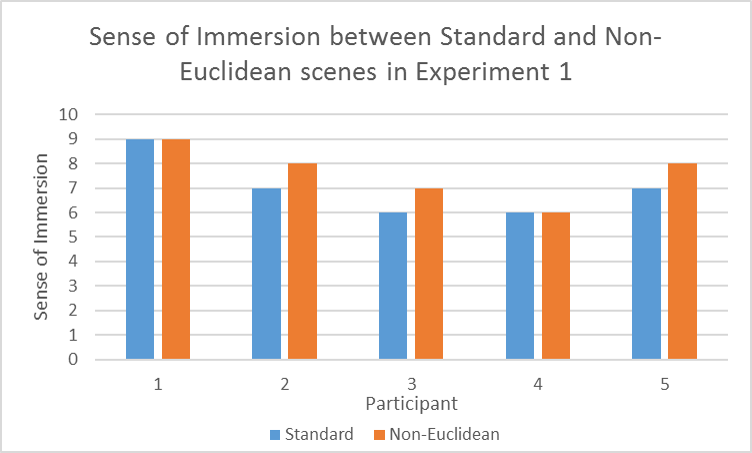
\includegraphics[width=0.7\textwidth]{Images/Compare_Immersion_Exp_1}
				\centering
				\caption{Comparison of participants sense of immersion in the two test scenes, from Experiment 1}
				\label{exp:fig:compare_immersion_exp1}
			\end{figure}

			\begin{figure}[H]
				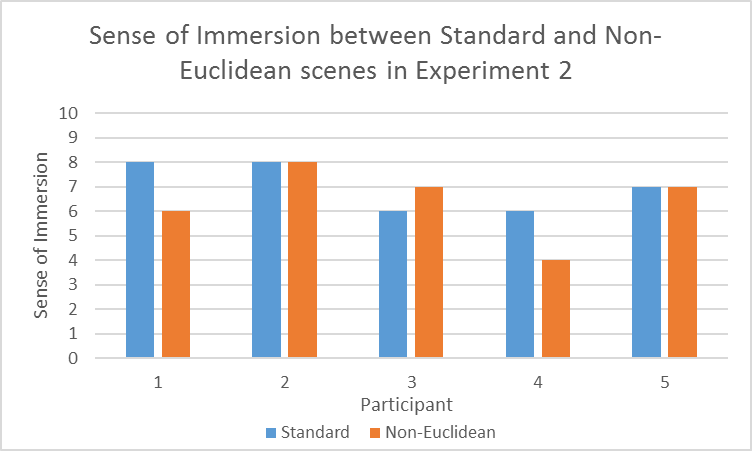
\includegraphics[width=0.7\textwidth]{Images/Compare_Immersion_Exp_2}
				\centering
				\caption{Comparison of participants sense of immersion in the two test scenes, from Experiment 2}
				\label{exp:fig:compare_immersion_exp2}
			\end{figure}

			\begin{figure}[H]
				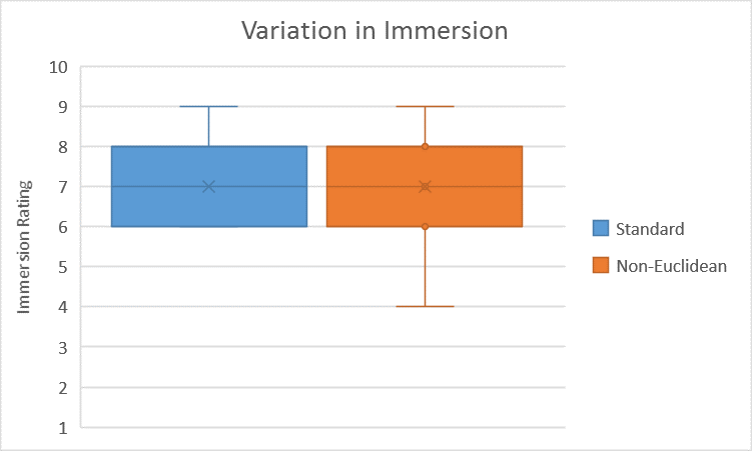
\includegraphics[width=0.7\textwidth]{Images/Compare_Immersion_Variation}
				\centering
				\caption{Mean values, and variation of Range for Immersion in the two test scenes}
				\label{exp:fig:compare_immersion_variation}
			\end{figure}

	\section{Summary}
	\label{exp:summary}

		The results of the experiments as a whole are interesting in the sense that they go against original expectations.

		% TODO - Here I will be evaluating the results of the experiments, covering any trends that appeared between the various experiments, discussing potential impacts from the results, as well as covering any additional notes that were provided about the experiments from the participants which weren't directly related to the specific experiment they were part of.

		% Results show that an NE environment can be more immersive than a standard env, so long as the user has had a chance to familiarise themselves in a standard euclid setting first
		% More work needs doing to improve upon the navigation side, there were mixed reviews from both scenes and experiments - quote feedback - room for further study

	
	% Project Evaluation
	\chapter{Project Evaluation}
\label{eval}

	\section[Scope]{Project Scope}

		The scope of this completed product and project as a whole differs to my proposed plan at the beginning of the year.
		The plan for this project was to study the effects tracking calibration of a VR headset has on a user outside of VR.
		However during the research stage for the project, existing studies were found which already covered the aspects I was planning on studying.
		The scope of this project came from combining my original proposal in the second year of creating a framework to build non-Euclidean virtual environments with the research I had found for VR.
		The decision to switch to this project instead of either of the originally proposed plans is one I am happy with.
		The scope of this project compared to the original ones is a lot more suitable for the time which was available for the project, and it is also a project which was more interesting to both design and conduct experiments for.

	\section[Implementation]{Product Implementation}

		The original plan for the product was to build an engine in DirectX 11 designed specifically for creating non-Euclidean environments.
		Although initial testing for the custom engine was promising, due to the scope of the features that would need to be implemented into it for it to be viable for the experiments, I decided to switch instead to an existing engine (Unity), which has the features which are not unique to the project built well already.
		The switch to the existing engine allowed me to focus more of my efforts on getting the non-Euclidean features of the product working well, and allowed me to use tools provided by Oculus for official support of the HMD which was to be used in the experiments.

		Using the existing engine for creating the product was not a perfect solution, however.
		The way in which the Oculus Rift SDK interacts with the Unity engine, while fine for Euclidean scenes, had minor issues when working with the implementation of non-Euclidean space made for this project.
		Although the implementation works perfectly fine when the HMD is not attached and it is being rendered direct to a regular monitor, the Oculus SDK modifies the depth and positioning of the cameras when rendering to the HMD, which sometimes caused slight gaps to appear between connected areas.
		I was able to minimise the impact it had by working around its offsets as best I could (See line 85 in \autoref{appendix:code:camera}), it was still noticed by a few of the participants in the experiments.

		Even though there were issues caused by the way the Oculus SDK positioned the cameras, I am happy with the way the implementation of the system turned out.
		When the system is being ran outside of the HMD, the rendering of the connections is seamless (As seen in \autoref{design:fig:game}), and when attempting to move between the two connected points, there is no indication to the player that they have moved anywhere other than where they expect.
		As well as this, the indicators in the scene view in the Unity editor that were added to the connection points worked very well, and were a great help when designing the scenes to be used for the experiments.

		In terms of how well used the system was for the scenes created for the experiments, I feel that I could have probably expanded the non-Euclidean scene to use more examples of the potential of the system.
		I do feel that the actual created scene was effective for its purpose in the experiment, however there are additional use cases I would have liked to have added, such as making the player appear to walk onto a different surface of the scene environment (such as a wall or roof), or perhaps scale the player so they are bigger or smaller when moving into a familiar space. % TODO: Reword this?

	\section{Experiment}

		

		% Talk about being happy with the amount of data you recieved, and how the results went against your original expectations for the results (which is a good thing!)

		

		% Talk about how you could have repeated the experiment with the feedback but with different navigation methods to see how that effects immersion - room for further study


	\section{Summary}

		As a whole I am happy with the outcome of the project.
		Overall it was well scoped for an initial endeavour into research in the subject area, giving possible areas for future expansion.
		There are areas in which I feel could have been expanded upon in the project, such as experimenting with different uses of non-Euclidean geometry, or increased sample sizes for participants of the experiments.
		The product itself, however, was executed well.
		The functionality it provided covered all of the use cases required to conduct the experiments, and did so efficiently, given the use case.

		% TODO: Reword, like, this entire section. It isn't that great.


	% Conclusion
	\chapter{Conclusion}
\label{conclusion}

	Here is where I will conclude the report as a whole, covering the results of the experiment, how they match up to the information learned from the existing literature review, as well as any further work which could be done on the subject area.


	% Bibliography
	\nocite{*}	% Make all entries in the bibliography file appear in the references section, even if not cited directly
	\begingroup
		\chapter{References}
		\label{ref}

		\renewcommand{\chapter}[2]{}		% Change chapter behaviour to make it not force the bibliography onto the following page
		\bibliographystyle{apalike}			% Set the bibliography to use APA formatting
		\bibliography{FinalYearProject}	    % Select the file to use for the bibliography
	\endgroup

	% Appendices
	\chapter{Appendix}
\label{appendix}

	% List of Figures
	\begingroup
		\section{List of Figures}
		\label{appendix:figures}

		Below are a list of the figures which are present in the document, along with their corresponding page number.

		\renewcommand{\chapter}[2]{}		% Change chapter behaviour to make it not force the list of figures onto the following page
		\listoffigures						% Display the list of figures
	\endgroup

	\section{Code Samples}
	\label{appendix:code}

		Below are code snippets for sections or complete functions that have specifically been referenced in the body of the report.
		The full source code and project can be found at the GitHub Repository here:

		\url{https://www.github.com/nboxhallburnett/IndividualProject}

		\begin{lstlisting}[caption="Camera Positioning - CameraRenderPosition.cs", label=appendix:code:camera, firstnumber=85]
Vector3 offset = PointOfView.position - _player.position + ((_player.position - _player.parent.parent.position) / 2);

// Position and rotate the cameras depending on the type of illusion they are going for
if (!Inverse) {
	Moveable.position = Helper.RotatePointAroundPivot(RenderPosition.position - offset, RenderPosition.position, _relativePortalRot.eulerAngles);
	Moveable.rotation = _relativePortalRot * Quaternion.Euler(rotationOffset + _defaultRot - _normalisedDefaultRot);
} else {
	Moveable.position = RenderPosition.position - offset;
	Moveable.rotation = _relativePortalRot * Quaternion.Euler((RenderPosition.transform.up == Vector3.up ? rotationOffset : -rotationOffset) + _defaultRot - _normalisedDefaultRot + new Vector3(0, 180f, 0));
}

// Set the near clipping plane of the camera to only render starting from the closest visible area
_cam.nearClipPlane = (Helper.FindClosestPoint(_bounds, transform.position) - transform.position).magnitude / 2f;
		\end{lstlisting}

		\begin{lstlisting}[caption="Player Positioning - CameraRenderPosition.cs", label=appendix:code:player, firstnumber=125]
/// <summary>
/// Re-Position the player from their current position to the equivelant position of its point of view, depending on their relative position
/// </summary>
/// <param name="player">Player to potentially transport</param>
/// <param name="centre">Centre of the currently colliding object</param>
/// <param name="forward">Forward vector of the currently colliding object</param>
public void positionPlayer (Collider player, Vector3 centre, Vector3 forward) {
	// Get the distance vector between the player and the centre of the currently colliding object
	Vector3 distance = player.transform.position - centre;
	Quaternion inverseFlip = Quaternion.Euler(0, 0, 0);

	// If only one of the points are inverted, make sure to flip the player
	if (Inverse != _linkedScript.Inverse) {
		inverseFlip = Quaternion.Euler(0, 180f, 0);
	}

	// If the player is more than half way through the object, transport them to the linked area
	if (Vector3.Dot(distance.normalized, forward) < 0) {
		// Set player position
		distance = Helper.RotatePointAroundPivot(distance, Vector3.zero, (_relativePlayerRot.eulerAngles + inverseFlip.eulerAngles));
		player.transform.position = PointOfView.position;
		player.transform.position += distance;

		// Set player rotation
		rotationOffset += _relativePlayerRot.eulerAngles + inverseFlip.eulerAngles;
		player.transform.rotation = _relativePlayerRot * inverseFlip * player.transform.rotation;

		// Update the players momentum
		_playerControl.UpdateMoveThrottle(_relativePlayerRot * inverseFlip * _playerControl.GetMoveThrottle());
	}
}
		\end{lstlisting}

	\section{Questionnaire}
		\label{appendix:question}
		A blank copy of the form used to gather the feedback discussed in Chapter \ref{exp} can be seen in the following two pages. Either the 1 or 2 were highlighted under the 'Experiment' section at the top of each page before being given to a participant. This was used as a reference for myself as to which experiment the form was for, without indicating to the participant the nature of the experiment.

		A digital transcription of the gathered data can be found in the \enquote{Raw Data} sheet in the \href{https://github.com/nboxhallburnett/IndividualProject/blob/master/Report/Resources/Feedback\%20Data.xlsx?raw=true}{\texttt{Report/Resources/Feedback Data.xlsx}} file inside the Git repository mentioned in \autoref{appendix:code}.
		The completed physical versions of the forms containing the raw data gathered are available upon request.

		\includepdf[pages={-},scale=1]{"Resources/Project Feedback Questionnaire"}

	\section{Ethics Review}
	\label{appendix:ethics}
		A completed and signed copy of the Project Ethical Review Form can be found on the following two pages.

		\includepdf[pages={-},scale=0.9]{"../Ethical Review Scan"}
		

% End the document
\end{document}
